\documentclass[a4paper,12pt,oneside]{report}

\usepackage[czech]{babel}
\usepackage[utf8]{inputenc}
\usepackage[T1]{fontenc}
\usepackage{lmodern}
\usepackage[hidelinks,pdfusetitle]{hyperref}
\usepackage{graphicx}
\usepackage{listings}
\usepackage{lstlinebgrd}
\usepackage{multirow}
\usepackage{float}
\usepackage{xcolor}
\usepackage[latte]{catppuccinpalette}
\usepackage{mathtools}
\usepackage{pdfpages}



\lstdefinestyle{C}{
  language={C},
  breaklines=true,
  showstringspaces=false,
  breakatwhitespace=true,
  tabsize=4,
  stringstyle = {\color{CtpGreen}},
  commentstyle={\color{CtpOverlay1}},
  basicstyle = {\small\color{CtpText}\ttfamily},
  keywordstyle = {\color{CtpMauve}},
  keywordstyle = [2]{\color{CtpBlue}},
  keywordstyle = [3]{\color{CtpYellow}},
  keywordstyle = [4]{\color{CtpLavender}},
  keywordstyle = [5]{\color{CtpPeach}},
  keywordstyle = [6]{\color{CtpTeal}},
  otherkeywords = {<, ||, =, ?,+},
  morekeywords = [2]{},
  morekeywords = [3]{},
  morekeywords = [4]{},
  morekeywords = [5]{self},
  morekeywords = [6]{<, ||, =, ?, *},
  backgroundcolor = {\color{CtpBase}},
  captionpos=b,
  numbers = left,
}

\lstset{style=C}

\begin{document}

\begin{titlepage}
	\Large
	\begin{center}
		\textsc{ZÁPADOČESKÁ UNIVERZITA V PLZNI}\\
		\textsc{Fakulta aplikovaných věd}\\
		Katedra informatiky a výpočetní techniky\\
		\vspace{.5cm}
		
\includegraphics[width=\textwidth]{pdfs/FAV_logo.pdf}
		\vspace{.5cm}
		\textsc{Programování v jazyce C}\\
		Semestrální práce\\
		\textbf{Č.3: Nástroj pro řešení úloh lineárního programování}
		\vfill
		\textsc{Antonín Hobl} \hfill A23B0306P\\
		\raggedleft\textsc{\today}
	\end{center}
\end{titlepage}

\tableofcontents

\chapter{Zadání}

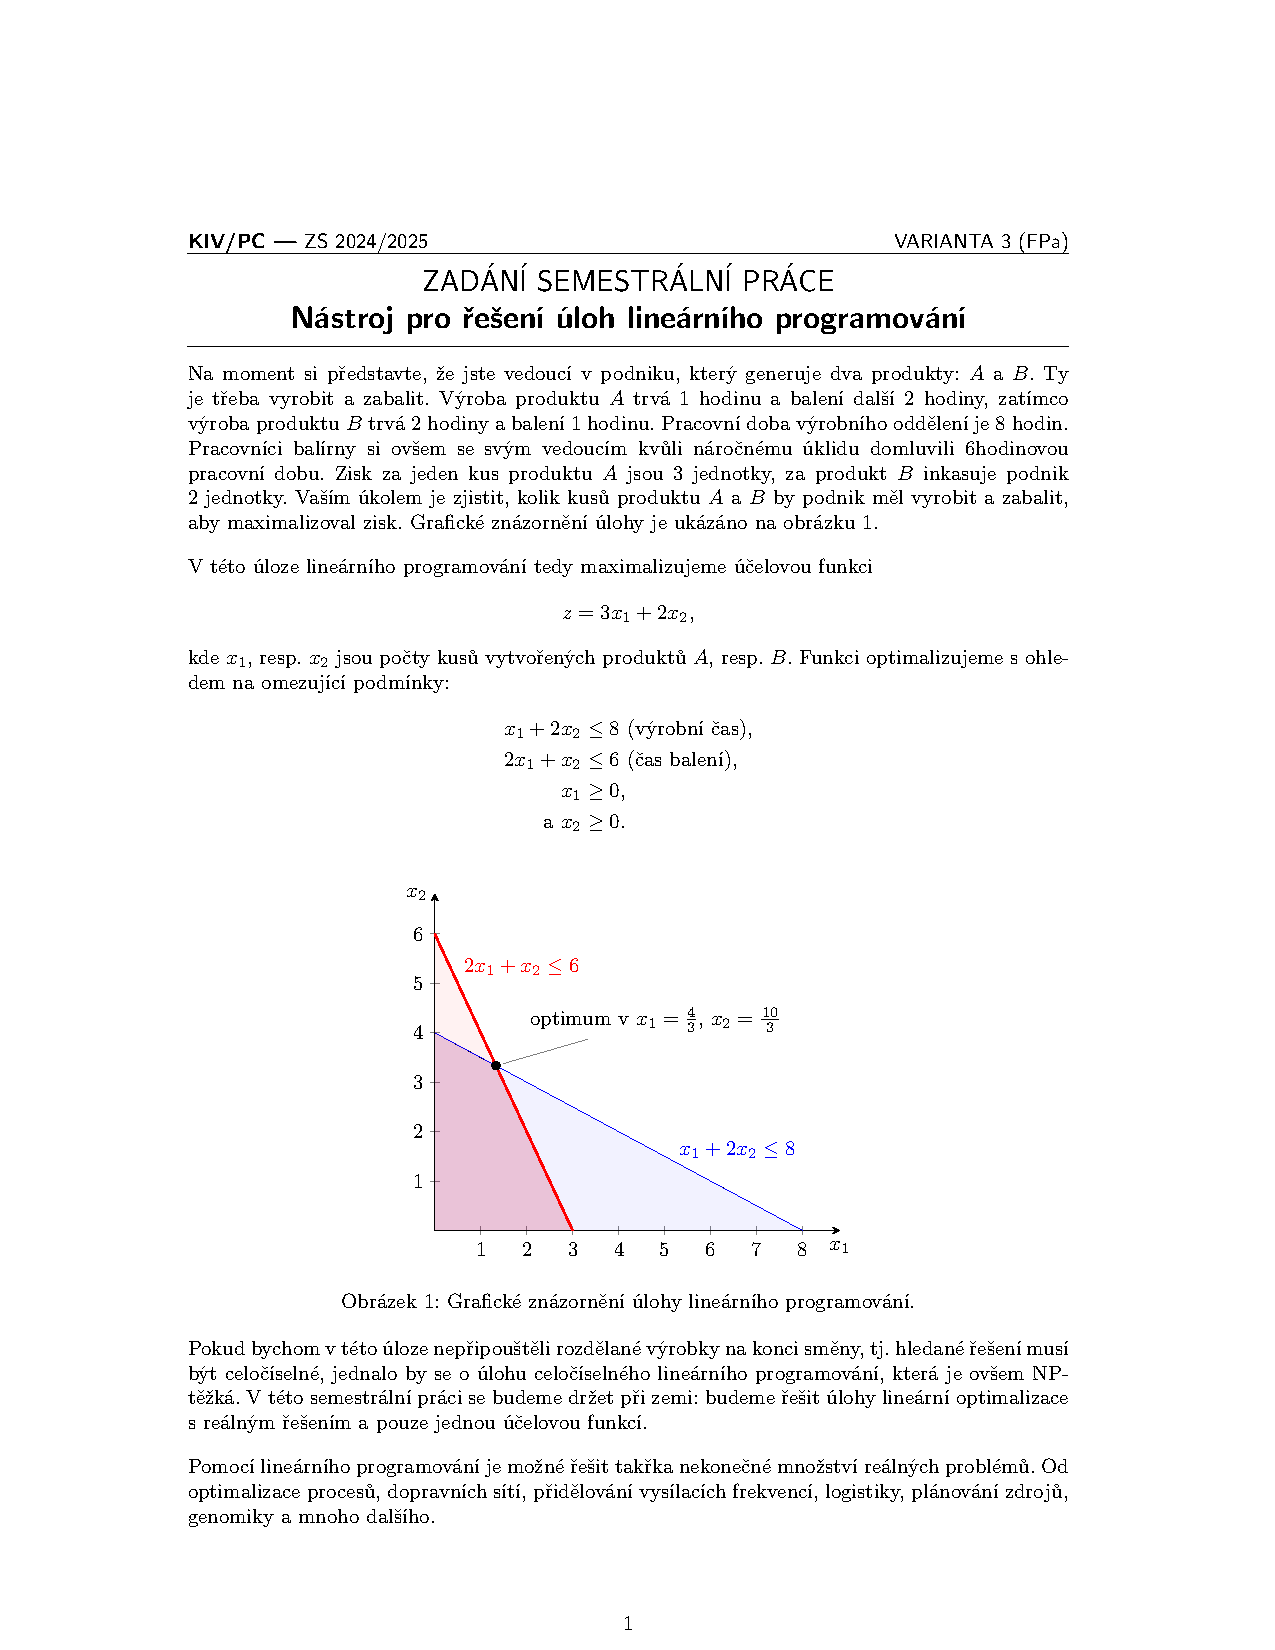
\includepdf[pages={-}]{zadani.pdf}

\chapter{Analýza úlohy}

V této kapitole bych chtěl popsat problémy, které přináší mnou vybrané zadání, nastínit možnosti jejich řešení a
ukázat, proč jsem si vybral to jedno konkrétní.

\section{Zpracování souboru}
Jako první problém nastalo samotné zpracování souboru. Problém byl, jak ho vlastně zpracovat, v jakém pořadí zpracovávat sekce, nebo jakým způsobem
jeho obsah vhodně uložit. Na stole jsem měl následnující možnosti.

\subsection{Zpracovávání souboru rovnou}
Jako první možnost bylo zpracovat soubor rovnou, to znamená postupně číst jeho řádky a z jednotlivých sekcí rovnou parsovat důležitá data a ukládat je do struktur.\par
Tahle možnost se zdá jako nejjednodušší, ale přináší s sebou problémy. Hlavní problém je, že nemáme zaručeno pořadí jednotlivých sekcí, to 
znamená, že pokud bychom se spoléhaly, že například sekce Generals bude jako první, tak by námi zvolený způsob nefungoval. Přesně tohle je hlavní 
problém tohoto řešení, protože na parsování dalších sekcí je potřeba základní seznam proměnných, tedy sekce Generals. My ale nemáme
zaručeno, že tato sekce bude v souboru jako první. Tento fakt velmi ztěžuje tuto možnost zpracování souboru a proto jsem se rozhodl ji nepoužít.

\subsection{Zpracovat nejdříve generals}
Druhá možnost byla zpracovat nejdříve sekci Generals a poté zbytek souboru. To znamená přečíst soubor jednou a vyparsovat z něj pouze
sekci Generals, kvůli seznamu proměnných, a uložit jej do struktury. Následně přečíst soubor znovu a zpracovat zbylé sekce souboru, kdy už 
bychom měli k dispozici seznam proměnných.\par Tahle možnost je lepší, neboť při zpracování zbylých sekcí budeme mít k dispozici nutný seznam proměnných.
Rozhodl jsem se ale tuto možnost zamítnout a to proto, že bych byl nucen číst soubor dvakrát a to mi přijde zbytečné.

\subsection{Rozdělit soubor podle sekcí}
Poslední možnost byla rozdělit soubor podle sekcí do struktury. To znamená číst soubor po řádkách a postupně, podle toho, na 
jaké sekce program narazí ukládat řádky jednotlivých sekcí do struktury, kde už bylo to bylo obsahově seřazeno podle sekcí.
Následně by bylo možné jednotlivé sekce zpracovat v libovolném pořadí a to bez nutnosti procházet soubor vícekrát. Tímhle máme 
zaručeno, že sekci Generals můžeme zpracovat jako první a při zpracování následujících sekcí budeme mít k dispozici seznam proměnných.\par
Tento způsob je sice složitější, ale nabízí velkou výhodu, a to zpracování sekcí v libovolném pořadí. Z toho důvodu jsem tento způsob zvolil
ve své implementaci.

\section{Zpracování aritmetického výrazu}

\section{Optimalitační algoritmus}

\chapter{Popis implementace}

\chapter{Uživatelská příručka}

\chapter{Závěr}

\end{document}
